\documentclass[12pt,letterpaper]{article}
\usepackage{preamble}

%%%%%%%%%%%%%%%%%%%%%%%%%%%%%%%%%%%%%%%%%%
%%%% Edit These for yourself
%%%%%%%%%%%%%%%%%%%%%%%%%%%%%%%%%%%%%%%%%%
\newcommand\course{Linear Control Theory}
\newcommand\hwnumber{1}
\newcommand\userID{Daniil Manakovskiy}
\newcommand\userGroup{BS18-02}

\begin{document}
Variant: C
\section*{Question 1}
\label{Q:1}
Given equation:
\begin{equation*}
    x'' + 2x' = -2x+3sin(t)
\end{equation*}
\begin{enumerate}[leftmargin=!,labelindent=5pt]
    \item Figure \ref{fig:1} demonstrates a solution of the $2^{nd}$ order differential equation in Simulink without using transfer func block. Figure \ref{fig:1_out} is a plot of simulation made by the scheme mentioned above.
        \begin{figure}[H]
            \centering
            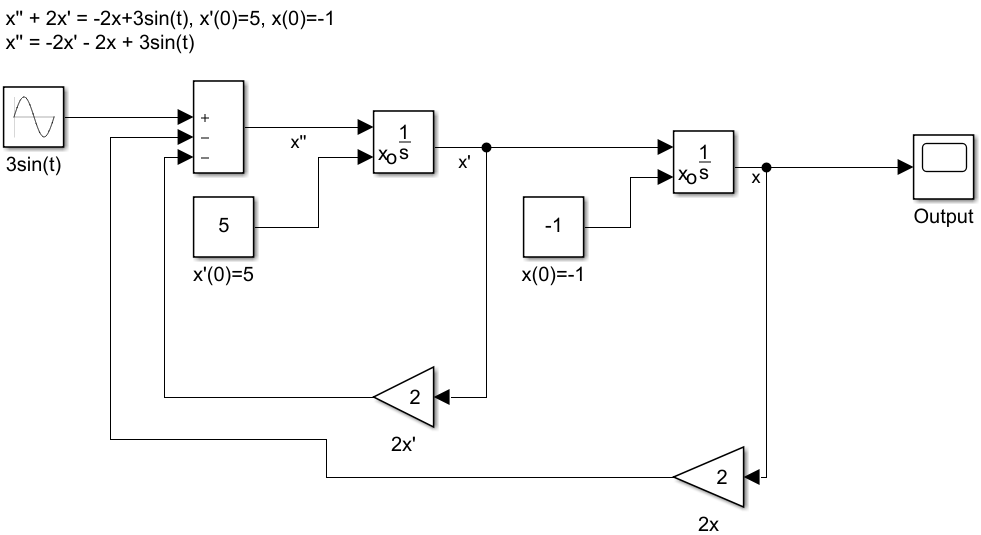
\includegraphics[width=15cm]{images/schemas/ex1_scheme.png}
            \caption{Simulink schema (without transfer func)}
            \label{fig:1}
        \end{figure}
        \begin{figure}[H]
            \centering
            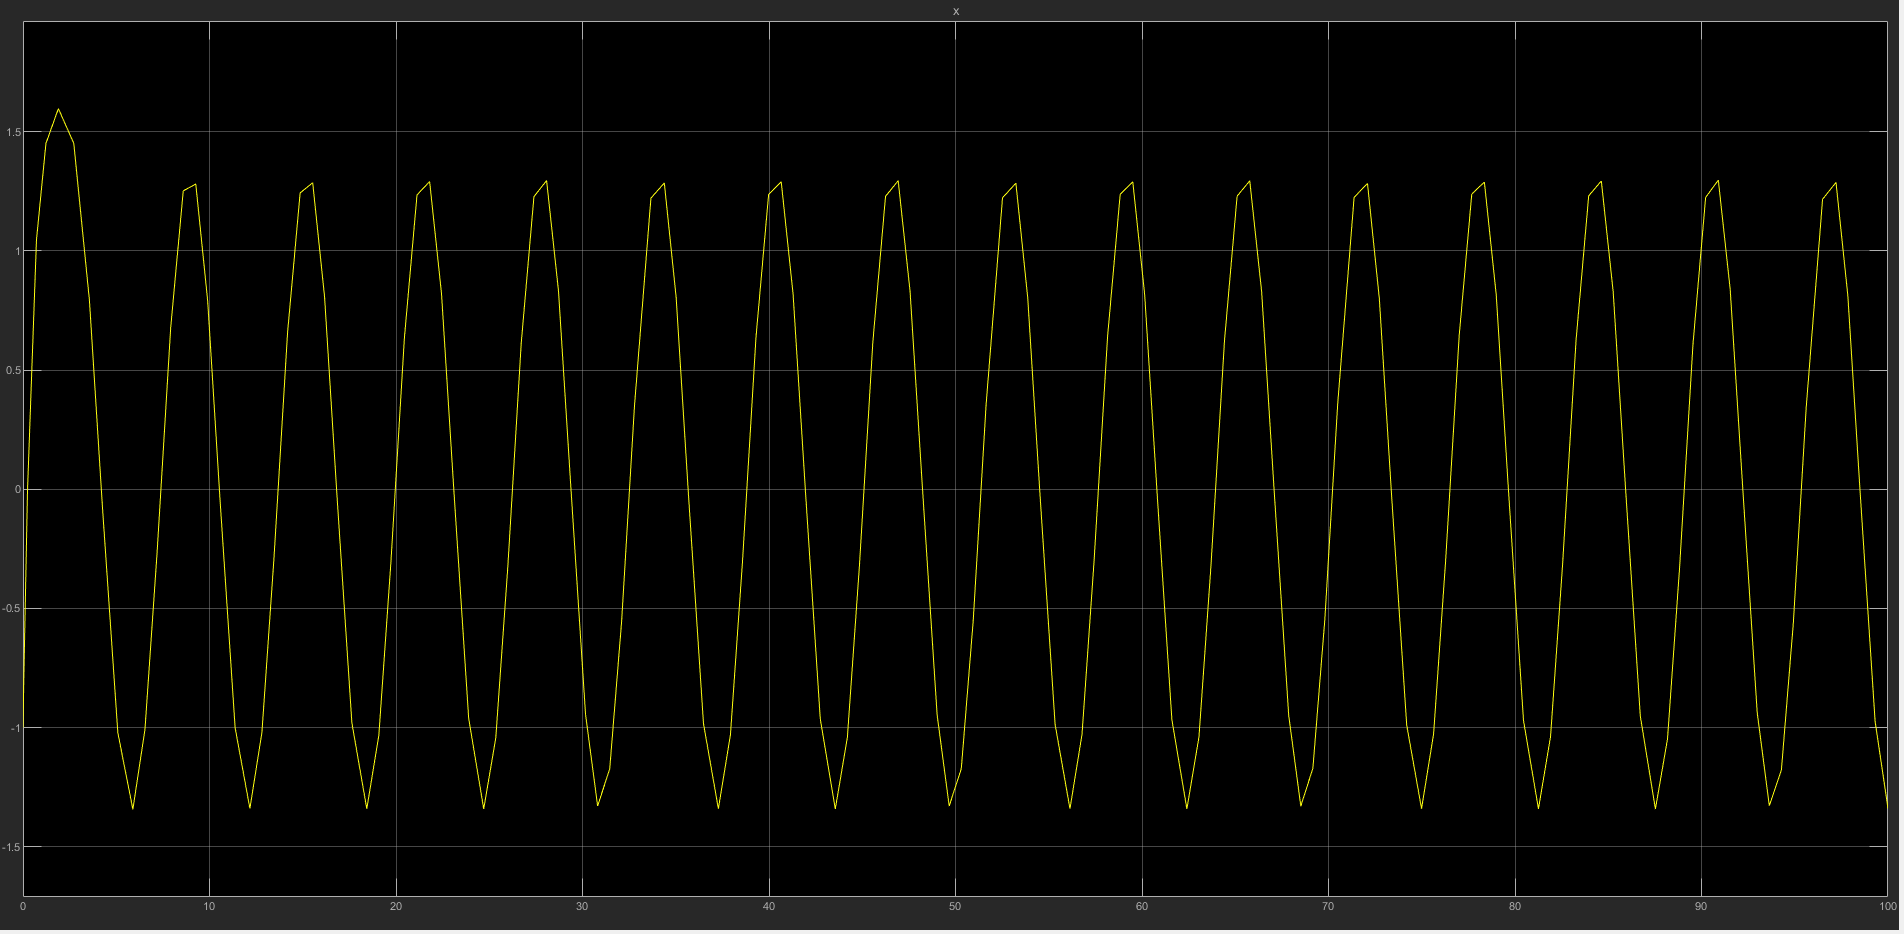
\includegraphics[width=15cm]{images/output/ex1_out.png}
            \caption{Simulink schema (without transfer func) output}
            \label{fig:1_out}
        \end{figure}
        
    \item Figures \ref{fig:2} and \ref{fig:2_out} shows the scheme and plot of the equation using transfer func block.The initial conditions were changed to zeros, since transfer function can't accept any ("Unfortunately, one can only solve problems with zero initial conditions" from 'Solving differential equations using simulink' by R. Herman, page 72)
    \begin{figure}[H]
            \centering
            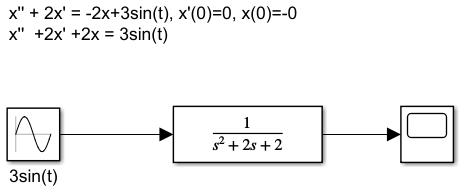
\includegraphics[width=15cm]{images/schemas/ex1_transfer_scheme.png}
            \caption{Simulink schema (with transfer func)}
            \label{fig:2}
        \end{figure}
    \begin{figure}[H]
            \centering
            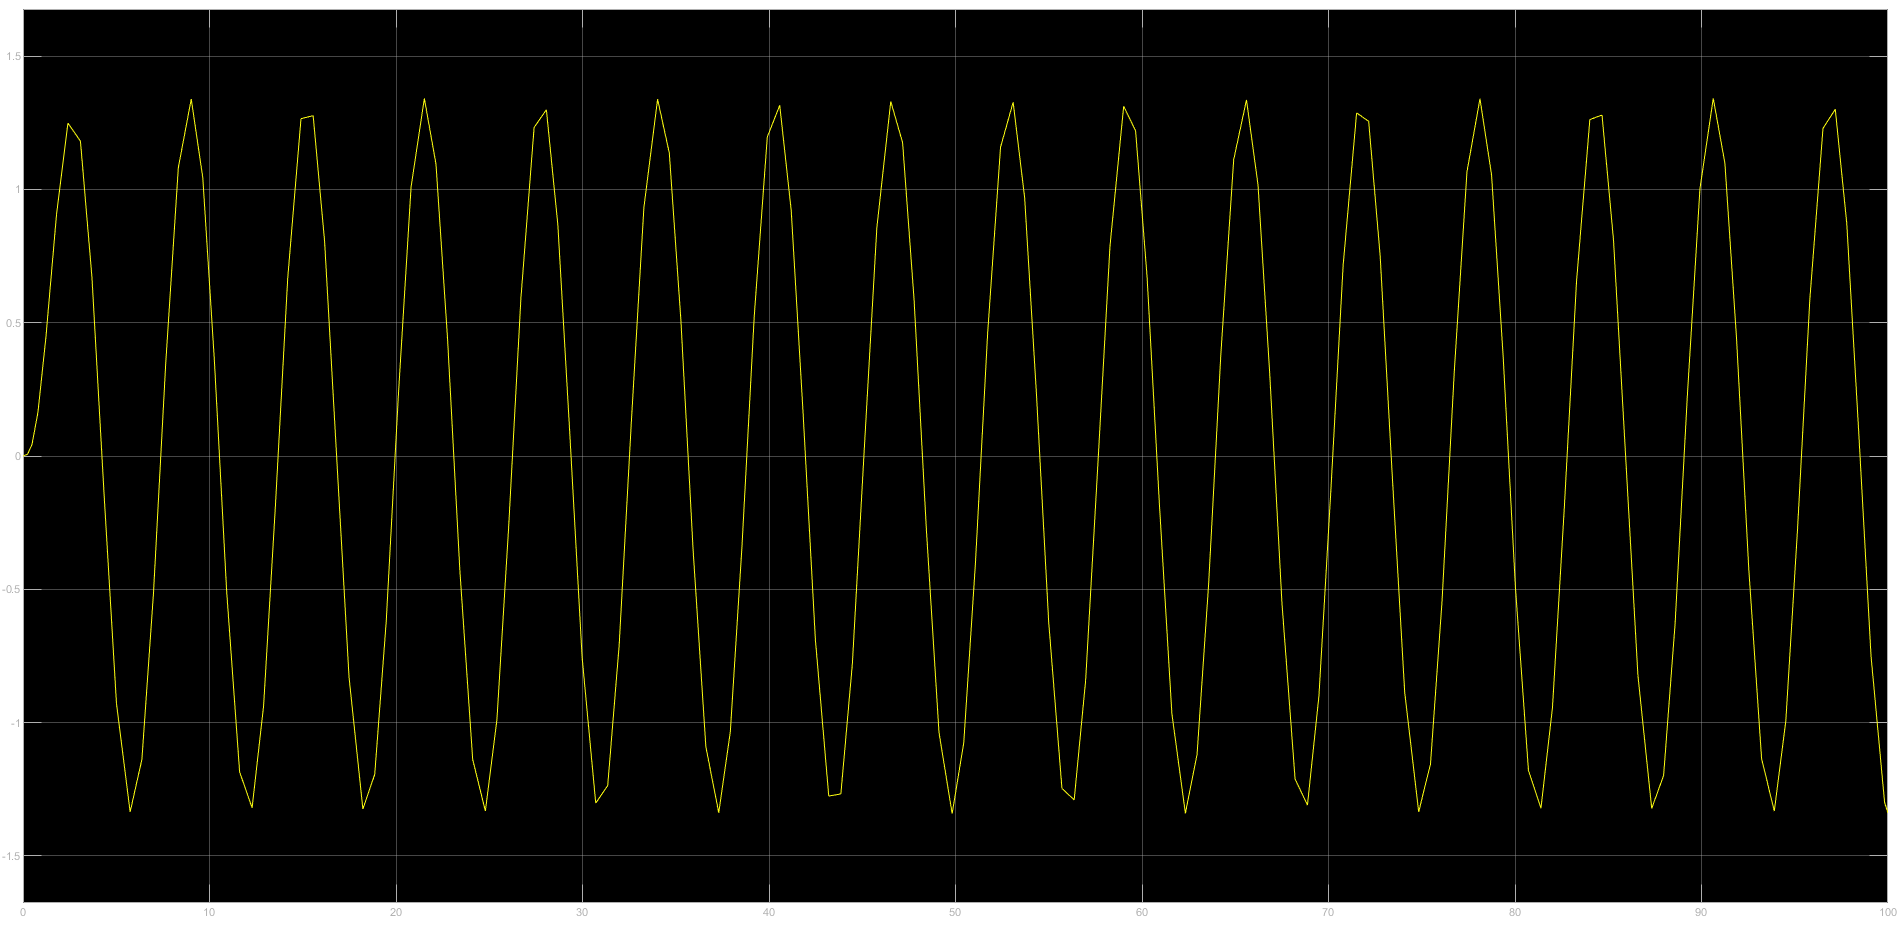
\includegraphics[width=15cm]{images/output/ex1_transfer_out.png}
            \caption{Simulink schema (with transfer func) output}
            \label{fig:2_out}
        \end{figure}
        
    \item Matlab code for solving the differential equation using Symbolic Toolbox is shown at listing \ref{code:dsolve}. Figure \ref{fig:dsolve_out} shows the graph of the solution.
        \lstinputlisting[caption={Matlab solution via dsolve}, label={code:dsolve}]{matlab_files/ex1_dsolve.m}
    \begin{figure}[H]
            \centering
            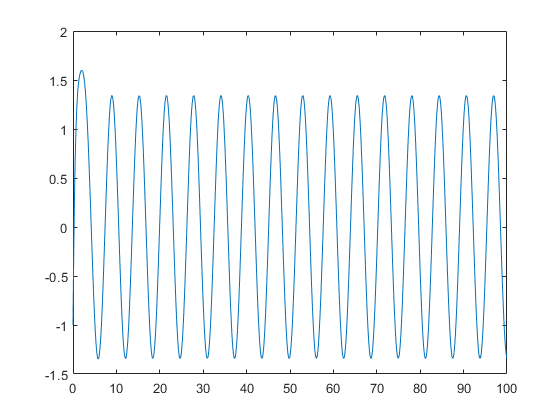
\includegraphics[width=15cm]{images/output/ex1_dsolve_out.png}
            \caption{Matlab solution (dsolve)}
            \label{fig:dsolve_out}
        \end{figure}

    \item Listing \ref{code:laplace} shows a solution using Laplace transform and Symbolic Toolbox. The graph is present on the figure \ref{fig:laplace_out}
        \lstinputlisting[caption={Matlab solution via transfer func}, label={code:laplace}]{matlab_files/ex1_laplace.m}
        \begin{figure}[H]
            \centering
            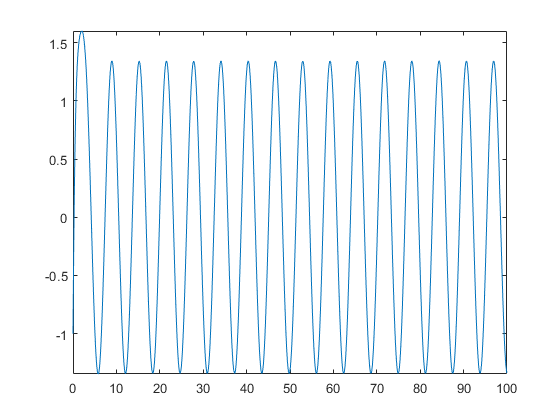
\includegraphics[width=15cm]{images/output/ex1_laplace_out.png}
            \caption{Matlab solution (dsolve)}
            \label{fig:laplace_out}
        \end{figure}
\end{enumerate}

\newpage
\section*{Question 2}
\setcounter{equation}{0}
\begin{enumerate}[leftmargin=!,labelindent=5pt]
     Find State Space Model of the system.
     \begin{equation*}
         x'' - x' +5 = t + 1\text{,  } y=2x+x'
     \end{equation*}
        
    \begin{equation*}
        x'' = x' - 4 + t
    \end{equation*}
   
   \begin{equation*}
        \begin{cases}
            \left[\begin{matrix}x'\\x''\end{matrix}\right] = 
            \left[\begin{matrix}0&1\\0&1\end{matrix}\right] \cdot 
            \left[\begin{matrix}x\\x'\end{matrix}\right] + 
            \left[\begin{matrix}0\\1\end{matrix}\right] \cdot (t-4) \\ 
         y = \left[\begin{matrix}2&1\end{matrix}\right] \cdot
        \left[\begin{matrix}x\\x'\end{matrix}\right] + 0 \cdot (t-4)
    \end{cases}
   \end{equation*}
\end{enumerate}


\section*{Question 3}
\setcounter{equation}{0}
\begin{enumerate}[leftmargin=!,labelindent=5pt]
    Find State Space Model of the system.
     \begin{equation*}
         2x^{(4)} + x^{(3)} - 3 x'' + 4x' -3 = u_1 - 2u_2\text{,  } y=4x'-u_1
     \end{equation*}
     \begin{equation*}
         x^{(4)} = -\frac{1}{2}x^{(3)} + \frac{3}{2}x'' -2x' + \frac{3}{2} + \frac{1}{2}u_1 - u_2
     \end{equation*}
     \begin{equation*}
         x^{(4)} = -\frac{1}{2}x^{(3)} + \frac{3}{2}x'' -2x'  + \frac{1}{2}u_1 - (u_2 - \frac{3}{2})
     \end{equation*}
     \begin{equation*}
         \begin{cases}
            \left[\begin{matrix}x'\\x''\\x^{(3)}\\x^{(4)}\end{matrix}\right] =
            \left[\begin{matrix}0&1&0&0\\0&0&1&0\\0&0&0&1\\0&-2&\frac{3}{2}&-\frac{1}{2}\end{matrix}\right] \cdot
            \left[\begin{matrix}x\\x'\\x''\\x^{(3)}\end{matrix}\right] + 
            \left[\begin{matrix}0&0\\0&0\\0&0\\\frac{1}{2}&-1\end{matrix}\right] \cdot
            \left[\begin{matrix}u_1\\u_2 - \frac{3}{2}\end{matrix}\right]
            \\
            y = \left[\begin{matrix}0&1&0&0\end{matrix}\right] \cdot
            \left[\begin{matrix}x\\x'\\x''\\x^{(3)}\end{matrix}\right] + 
            \left[\begin{matrix}-1&0\end{matrix}\right] \cdot
            \left[\begin{matrix}u_1\\u_2 - \frac{3}{2}\end{matrix}\right]
         \end{cases}
     \end{equation*}
\end{enumerate}

\section*{Question 4}
\setcounter{equation}{0}
\begin{enumerate}[leftmargin=!,labelindent=5pt]
    Write a function in python that converts any ODE of power n to the state space representation. \\
    
    ODE form:
    \begin{equation*}
        a_{k}y^{(k)} + a_{k-1}y^{(k-1)} + \dots + a_2 y'' + a_1 y' + a_0 y' = b_0
    \end{equation*}
    Desired output format: 
    \begin{equation*}
        \left[\begin{matrix}y'\\y''\\\vdots\\y^{(k)}\end{matrix}\right] = 
        \left[\begin{matrix}0&1&0&\dots&0&0\\0&0&1&\dots&0&0\\0&0&0&\dots&0&0\\\vdots&\vdots&\vdots&\ddots&\vdots&\vdots\\0&0&0&\dots&0&1\\-\frac{a_0}{a_k}&-\frac{a_1}{a_k}&-\frac{a_2}{a_k}&\dots&-\frac{a_{k-1}}{a_k}&-\frac{a_{k-1}}{a_k}\end{matrix}\right] \cdot
        \left[\begin{matrix}y\\y'\\y''\\\vdots\\y^{(n-2)}\\y^{(n-1)}\end{matrix}\right] + 
        \left[\begin{matrix}0\\0\\0\\\vdots\\0\\\frac{1}{a_k}\end{matrix}\right] b_0
    \end{equation*}
    The solution is presented at listing \ref{code:SS_ODE}. Usage: listing \ref{code:SS_ODE_usage}. Output example:
    \begin{verbatim}
Coefficients:  [0.99886853 0.92023046 0.75979535 0.66250064 0.7541122  0.52864808 
 0.73775728]
State:
[
 [ 0.          1.          0.          0.          0.          0.        ]
 [ 0.          0.          1.          0.          0.          0.        ]
 [ 0.          0.          0.          1.          0.          0.        ]
 [ 0.          0.          0.          0.          1.          0.        ]
 [ 0.          0.          0.          0.          0.          1.        ]
 [-0.73859298 -0.5292469  -0.75496643 -0.66325109 -0.76065601 -0.92127285]
] 
input_matrix:
 [0.         0.         0.         0.         0.         1.00113276]
    \end{verbatim}
    \lstinputlisting[language=Python,caption={Converting an ODE of degree n to StateSpace format}, label={code:SS_ODE}, linerange={1-26}]{python_code/StateSpaceReprODE.py}
    
    \lstinputlisting[language=Python,caption={Usage of constructStateSpace func.}, label={code:SS_ODE_usage}, linerange={27-33}]{python_code/StateSpaceReprODE.py}
\end{enumerate}

\section*{Question 5}
\setcounter{equation}{0}
\begin{enumerate}[leftmargin=!,labelindent=5pt]
    \item Write function in python that solves ODE.
    Since the ODE's order is n, solving technique is very similar to StateSpace, therefore some variables will be used from the state matrix. The code is on listing \ref{code:ODE_solve}. 
    \lstinputlisting[language=Python,caption={Solving linear ODE}, label={code:ODE_solve}, linerange={34-41, 49-52,60-71}]{python_code/StateSpaceReprODE.py}
    
    \item Write functions in python that solves ODE's state space representation.\\
    The function is presented at listing \ref{code:SS_ODE_solve}
    \lstinputlisting[language=Python,caption={Usage of constructStateSpace func.}, label={code:SS_ODE_solve}, linerange={34-41, 47-58}]{python_code/StateSpaceReprODE.py}
    
    \item Test functions on equations of task 2 (\nameref{Q:1}).
    \begin{enumerate}
        \item Output is presented at figure \ref{fig:ODE_plot}.
             \begin{figure}[H]
                 \centering
                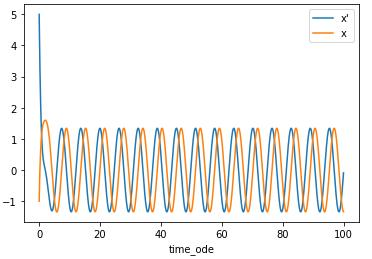
\includegraphics[width=15cm]{images/output/ode.jpg}
                \caption{ODE solution of \nameref{Q:1}}
                \label{fig:ODE_plot}
            \end{figure}
        \item StateSpace representation output at figure \ref{fig:SS_ODE_plot}
            \begin{figure}[H]
            \centering
            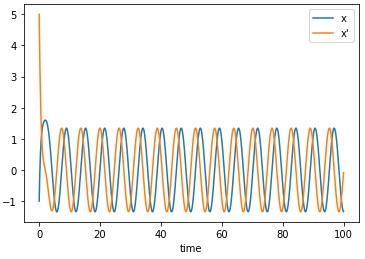
\includegraphics[width=15cm]{images/output/SS_ODE_plot.jpg}
            \caption{StateSpace representation solution of \nameref{Q:1}}
            \label{fig:SS_ODE_plot}
        \end{figure}
        
        Since the right-hand size contains the side the function of time, eigen-values can't tell anything about stability of a system. According to the plot \ref{fig:SS_ODE_plot}, the solution is stable, but diverges.
    \end{enumerate}
\end{enumerate}
\end{document}
